\documentclass[11pt,a4paper]{article}
\usepackage{amsmath}
\usepackage{amssymb}
\usepackage{graphicx}
\usepackage{subfigure}
\usepackage{float}
\usepackage{xeCJK}
\usepackage{geometry}
\geometry{left=2.0cm,right=2.0cm,top=2.0cm,bottom=2.0cm}

\title{基于五场朗道流体的误差场渗透模拟}
\author{任广智}
\date{\today}

\begin{document}

\maketitle

思路: 边界的磁扰动渗透会影响等离子体的旋转以及激发撕裂模,旋转的降低以及撕裂模的激发都会对湍流输运产生一定的影响。首先从两场出发,验证误差场渗透的参数和现象,然后考虑五场下密度和温度剖面的影响,注意一下异同,以及相关的输运特性和剖面变化。最后考虑温度激发强ITG湍流时候的激发情况。
\part{两场单流体模拟}

\begin{itemize}
	\item 约化MHD,单流体假设,不考虑压强剖面带来的抗磁性漂移以及不稳定性。
	\item 采用$(r,\theta,\zeta)$坐标系,但实际上没有考虑环效应。
	\item 只取了$(m/n)=(2/1)$模式演示,实际多螺旋的效果大致相同,区别不大。
\end{itemize}
	
\section{初始设置}
	\begin{itemize}
	\item 平衡磁场
		$$ q = \frac{3(1+f)}{4-6r^2+4r^4-r^6} $$
		其中$f = A(r-r_s)\exp(-[(r-r_s)/\delta]^2),r_s=0.811,\delta=0.05$。选取$A=0,0.01,0.05,0.1$得到不同$\Delta'_{2/1} = -0.13,0.5,3,6$的一组剖面,其中$A=0$时对应的平衡磁场由电流剖面$J_\zeta=J_0(1-r^2)^3$给出,$(m/n)=(2,1)$模有理面位置为$r_s=0.811$处。
	\item 极向旋转
		$$V_\theta = V_0\cdot r(1-r)/(1-r_s) $$
		这里$V_0$在后边的模拟中一般取3左右的数值大小,我认为这在$\beta$取0.1 \%时候是合理的,相当于旋转速度为百分之几的Alven速度。
	\item 粘滞系数
		$$\beta=0.001,D_U=10^{-2},\eta=5\times10^{-4}$$
		相当于
		$$ Lundquist\ number\ S=\frac{Lv_A}{\eta}=6.4\times{10^6} $$
	\item 边界磁扰动
		$$ \psi|_{r=a} = \psi_a\cdot\psi_{eq}|_{r=a}\exp(im\theta-in\zeta) $$
	\end{itemize}

\section{$\Delta'<0$时误差场引起的受迫磁重联}
	\begin{itemize}
	\item 不同边界磁扰动下磁岛的演化以及饱和磁岛宽度与边界磁扰动大小的关系:
		$$ V_0=3.0, \psi_a=1\times 10^{-5} \sim 1\times 10^{-3} $$
    	\begin{figure}[H]
		\centering
		\subfigure[磁岛宽度 vs. 时间]{
			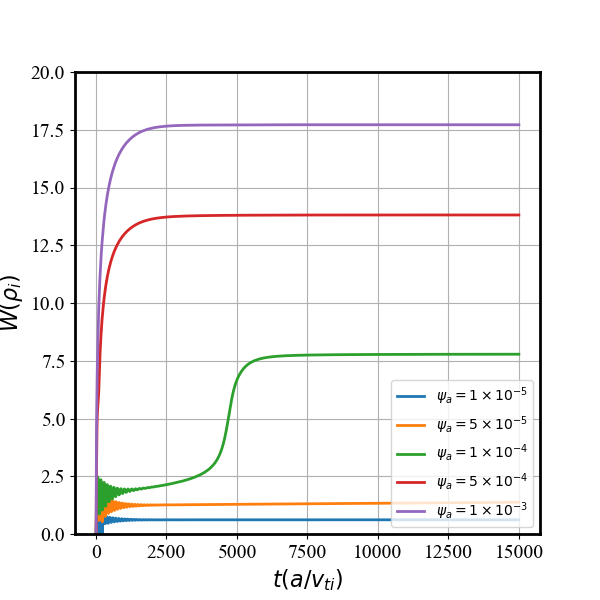
\includegraphics[width=0.35\textwidth]{../error_field/2f_stable/w_t_psi.png} 
		}
		\subfigure[磁岛宽度 vs. $\psi_a$]{
			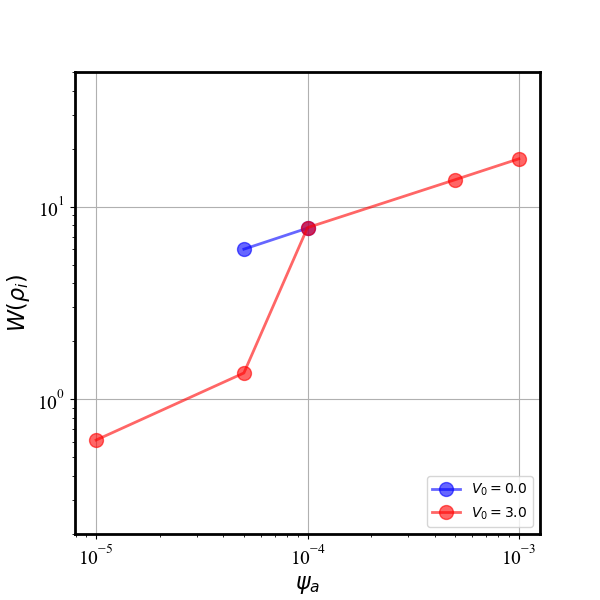
\includegraphics[width=0.35\textwidth]{../error_field/2f_stable/sw_psi.png}
		}
		\caption{}
		\end{figure}

	\item 不同旋转大小下磁场演化以及有理面处的极向旋转演化:
		$$ \psi_a =1\times 10^{-4}, V_0=3.0,5.0  $$
	    \begin{figure}[H]
		\centering
		\subfigure[磁岛宽度 vs. 时间]{
			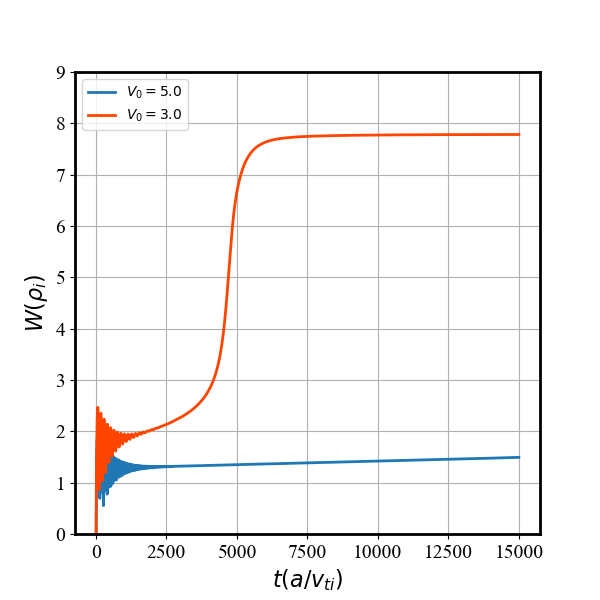
\includegraphics[width=0.35\textwidth]{../error_field/2f_stable/w_t.png} 
		}
		\subfigure[有理面处极向旋转 vs. 时间]{
			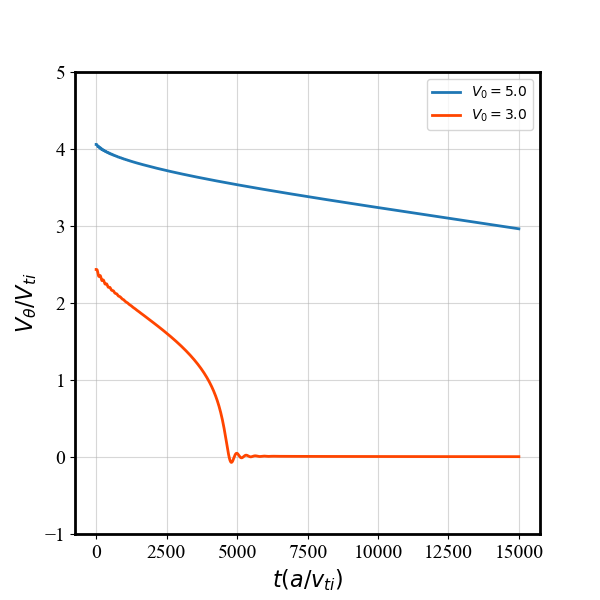
\includegraphics[width=0.35\textwidth]{../error_field/2f_stable/v_t.png}
		}
		\caption{}
		\end{figure}

	\item 不同旋转大小下稳态磁岛宽度以及旋转大小:
		$$ \psi_a =1\times 10^{-4}, V_0=-7\sim 7  $$
	    \begin{figure}[H]
		\centering
		\subfigure[稳态磁岛宽度 vs. $V_0$]{
			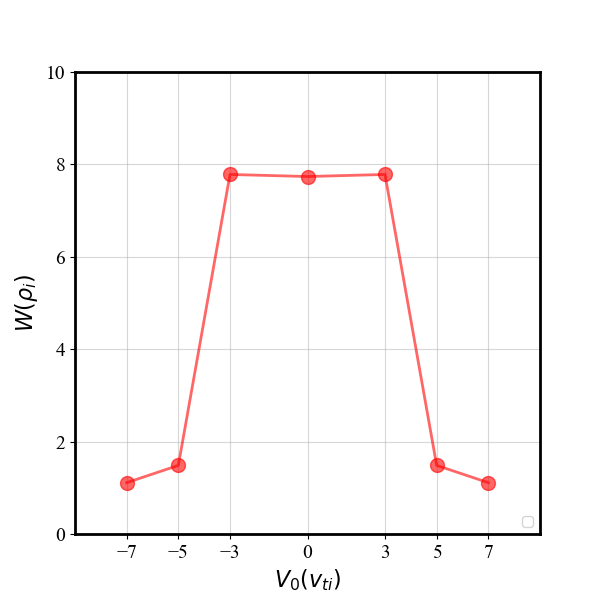
\includegraphics[width=0.35\textwidth]{../error_field/2f_stable/sw_v.png} 
		}
		\subfigure[稳态时有理面处极向旋转 vs. $V_0$]{
			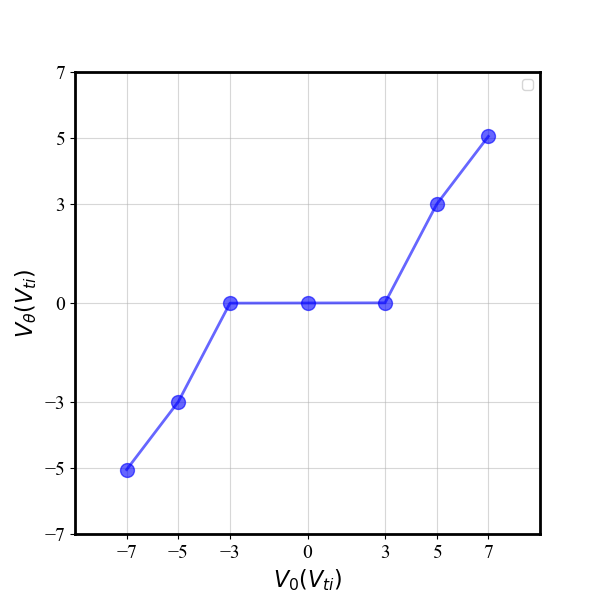
\includegraphics[width=0.35\textwidth]{../error_field/2f_stable/sv_v.png}
		}
		\caption{}
		\end{figure}
	
	\item 不同时刻2/1本征模结构和旋转剖面:
		$$ \psi_a =1\times 10^{-4}, V_0=3.0 $$
		\begin{figure}[H]
		\centering
		\subfigure[本征模结构]{
			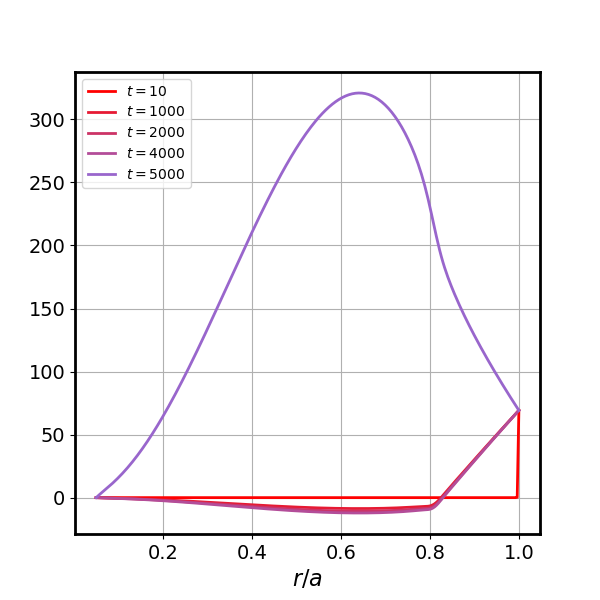
\includegraphics[width=0.35\textwidth]{../error_field/2f_stable/eig.png} 
		}
		\subfigure[极向旋转剖面]{
			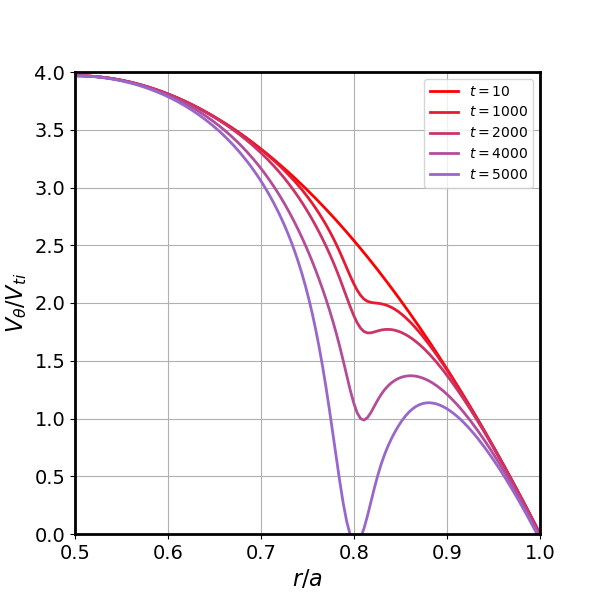
\includegraphics[width=0.35\textwidth]{../error_field/2f_stable/v_x.png}
		}
		\caption{}		
		\end{figure}		

	\end{itemize}

	总结: 
	1. 比较好地重复了别人柱位形下的工作
	2. 极向旋转对于误差场的渗透具有一定的屏蔽作用,边界的磁扰动的渗透会造成有理面处的锁模以及快速激发撕裂模。


\part{五场双流体模拟}

\begin{itemize}
	\item 五场程序目前对于$(1,0)$模式和zonal field并存下的结果不好,不能达到长时间的演化。
	\item 不考虑$(0,0)$模式的曲率耦合,即不考虑$(1,0)$
 	\item 对于$n=1$的模式只考虑$(2,1)$模
	\item 湍流为环形ITG激发的湍流
	\item 初始旋转的添加实际上是$E\times B$流的添加,即径向电场的添加,双流体下需要考虑抗磁性漂移和电漂移的共同作用
\end{itemize}

\section{平坦的压强剖面}
\begin{itemize}	
	\item 两场的ZF并没有单独来解,这里先测试一下五场时两种不同解法下是否有差别,以下是动能的演化以及磁岛宽度的演化:
		\begin{figure}[H]
		\centering
		\subfigure[动能]{
			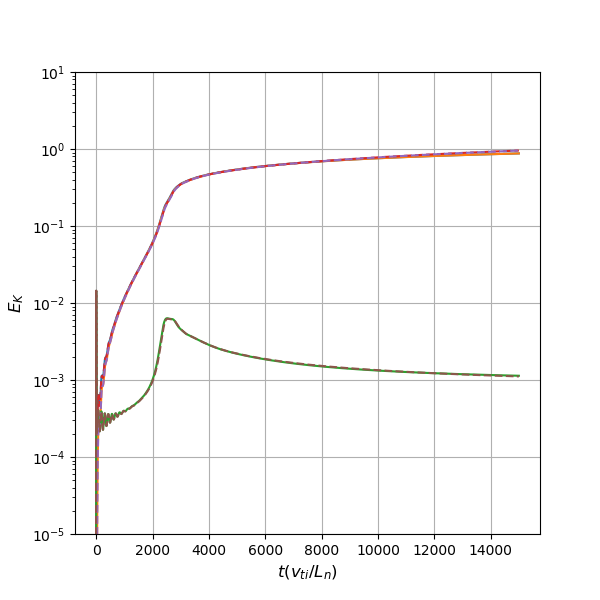
\includegraphics[width=0.35\textwidth]{../error_field/5f-0n0t/Ek_zf.png} 
		}
		\subfigure[磁岛宽度]{
			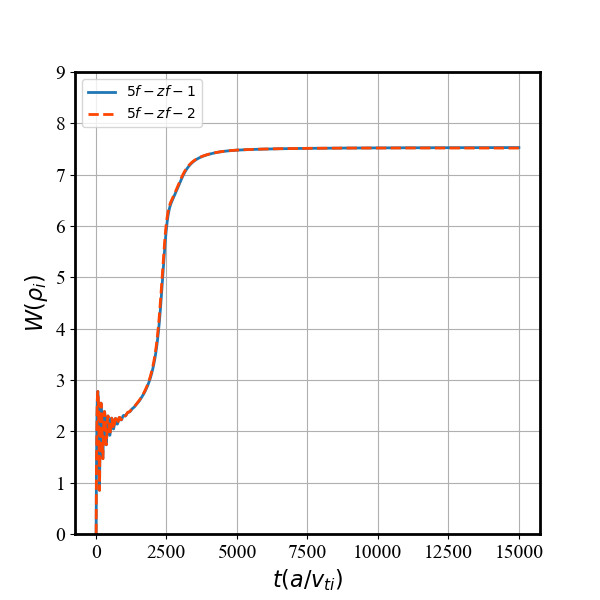
\includegraphics[width=0.35\textwidth]{../error_field/5f-0n0t/w_zf.png}
		}
		\caption{}		
		\end{figure}
	可以看出两种解法没有太大的差别,也说明了zf单独解的正确性
	
	\item 单模和多模的区别
		\begin{figure}[H]
		\centering
		\subfigure[动能]{
			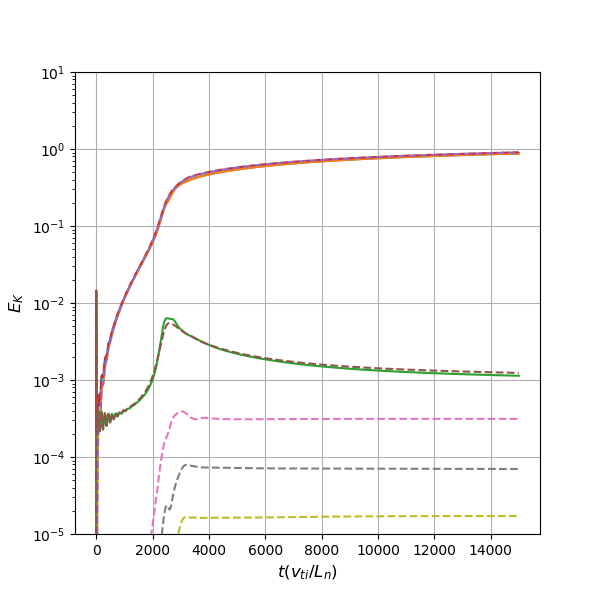
\includegraphics[width=0.35\textwidth]{../error_field/5f-0n0t/Ek_mn.png} 
		}
		\subfigure[磁岛宽度]{
			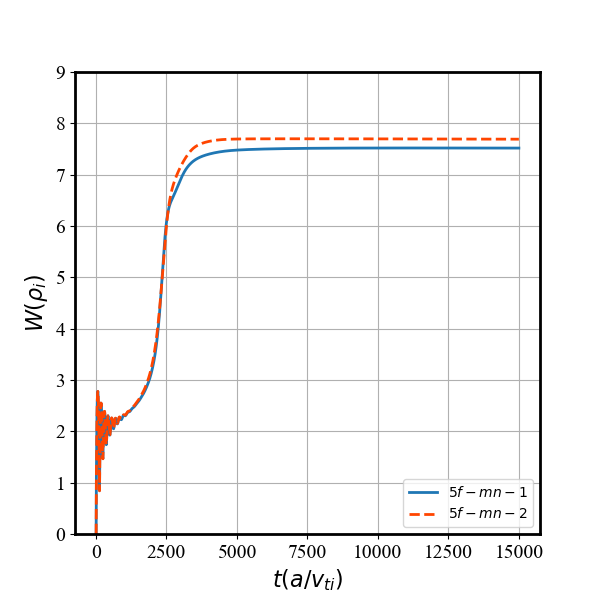
\includegraphics[width=0.35\textwidth]{../error_field/5f-0n0t/w_mn.png}
		}
		\caption{}		
		\end{figure}
	饱和磁岛宽度略有差别,演化趋势以及渗透阈值都变化不大,可以先用单模计算来找一下参数看一下变化
	
	\item 验证5场下磁岛与边界磁扰动的定标关系:
		\begin{figure}[H]
		\centering
		\subfigure[动能]{
			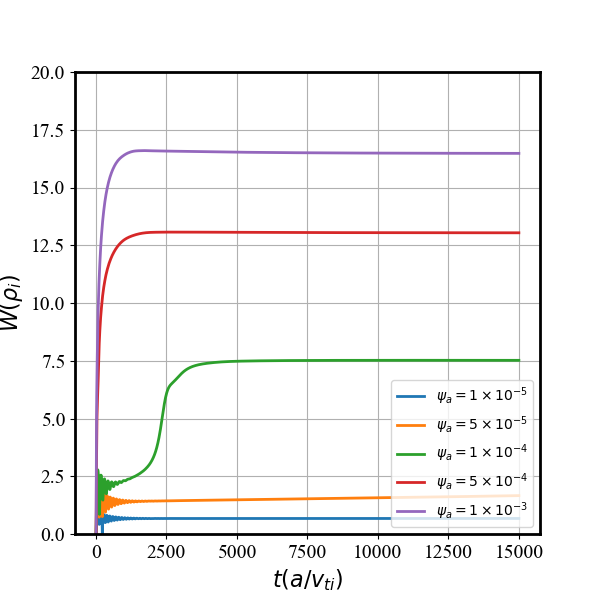
\includegraphics[width=0.35\textwidth]{../error_field/5f-0n0t/w_t_v.png} 
		}
		\subfigure[磁岛宽度]{
			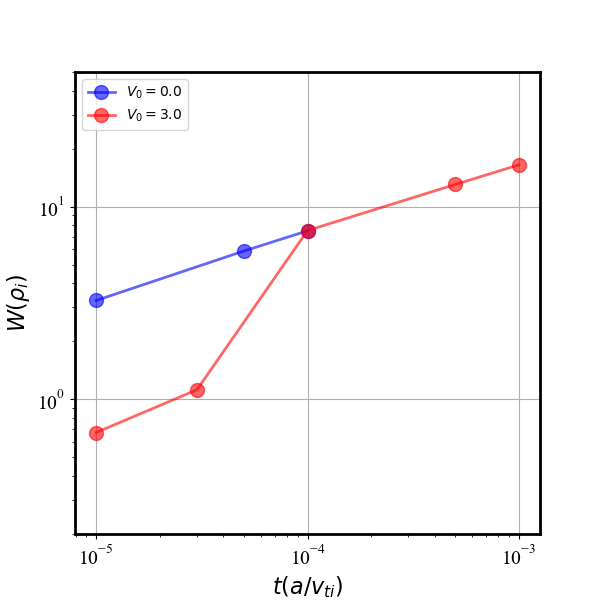
\includegraphics[width=0.35\textwidth]{../error_field/5f-0n0t/sw_psi.png}
		}
		\caption{}		
		\end{figure}
	饱和磁岛宽度略有差别,演化趋势以及渗透阈值都变化不大,可以先用单模计算来找一下参数看一下变化
	
	\item 对比两场和五场下的磁场宽度以及有理面处旋转的演化:
	\begin{figure}[H]
		\centering
		\subfigure[磁岛宽度]{
			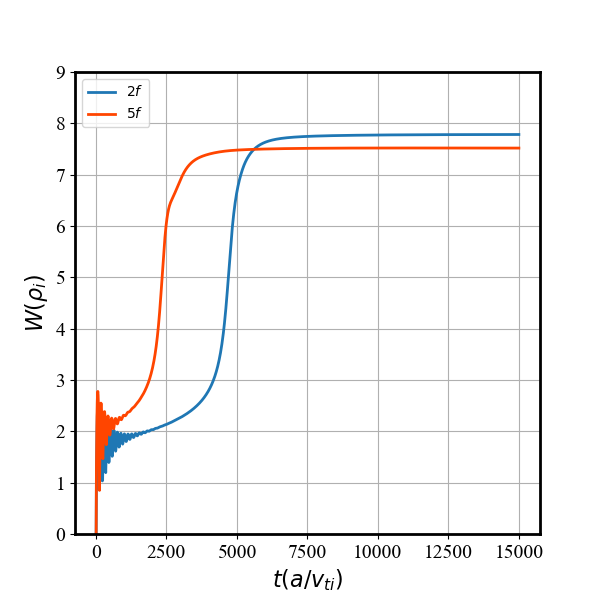
\includegraphics[width=0.35\textwidth]{../error_field/5f-0n0t/w_t.png} 
		}
		\subfigure[极向旋转]{
			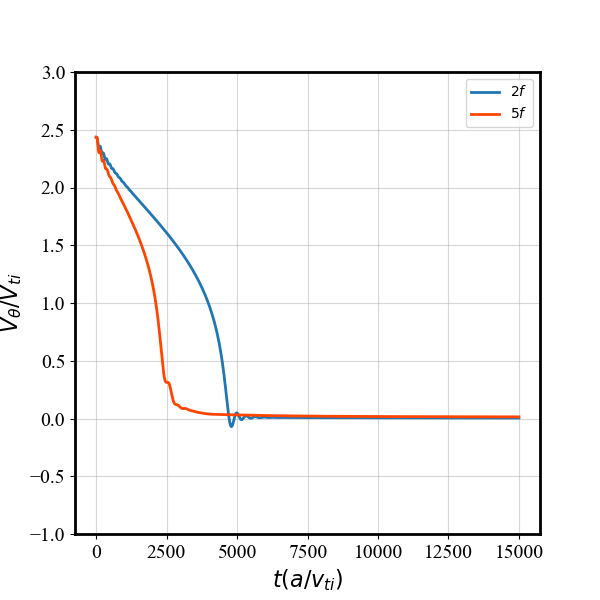
\includegraphics[width=0.35\textwidth]{../error_field/5f-0n0t/vy_t.png}
		}
		\caption{}		
	\end{figure}
	考虑双流体效应之后,误差场更快地渗透并且激发撕裂模,但是磁岛的饱和幅度比两场的稍小一点。
	
	\item  饱和磁岛宽度和旋转的关系
	\begin{figure}[H]
		\centering
		\subfigure[磁岛宽度]{
			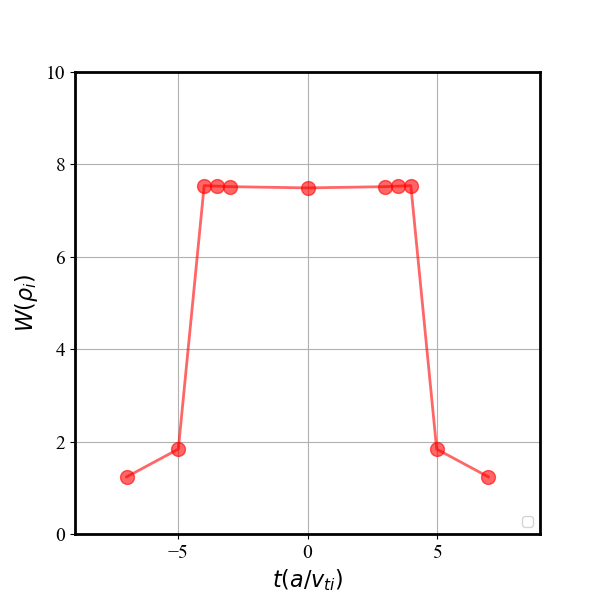
\includegraphics[width=0.35\textwidth]{../error_field/5f-0n0t/sw_v.png} 
		}
		\subfigure[极向旋转]{
			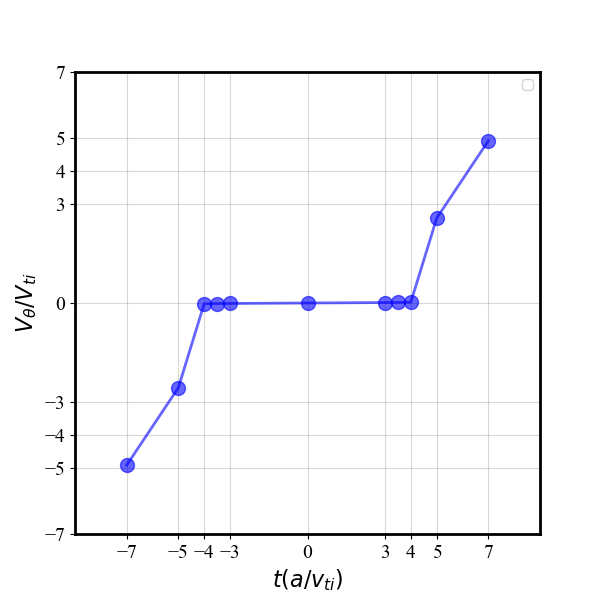
\includegraphics[width=0.35\textwidth]{../error_field/5f-0n0t/sv_v.png}
		}
		\caption{}		
	\end{figure}
	跟两场的结果保持大致的一致性
	
\end{itemize}


\section{平坦的温度剖面}
密度剖面:
$$ n = 0.7 + 0.3(1-(r/a)^2)^2 $$
\begin{itemize}
	\item 固定的密度剖面
	\begin{figure}[H]
		\centering
		\subfigure[磁岛宽度]{
			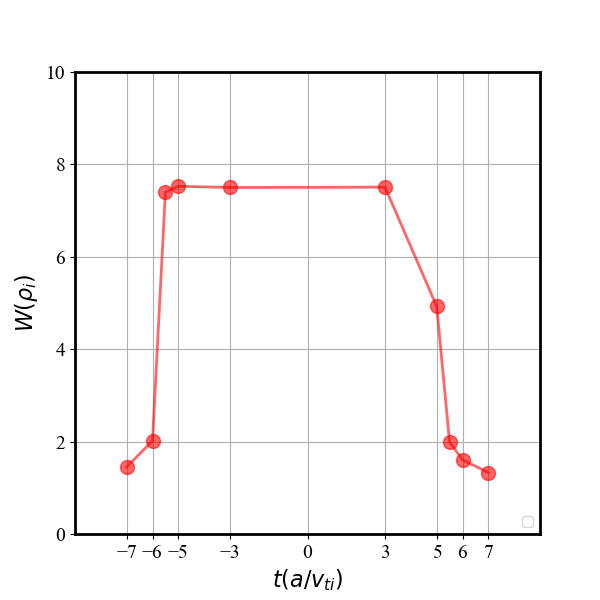
\includegraphics[width=0.35\textwidth]{../error_field/5f-1n0t/fix_n/sw_v.png} 
		}
		\subfigure[极向旋转]{
			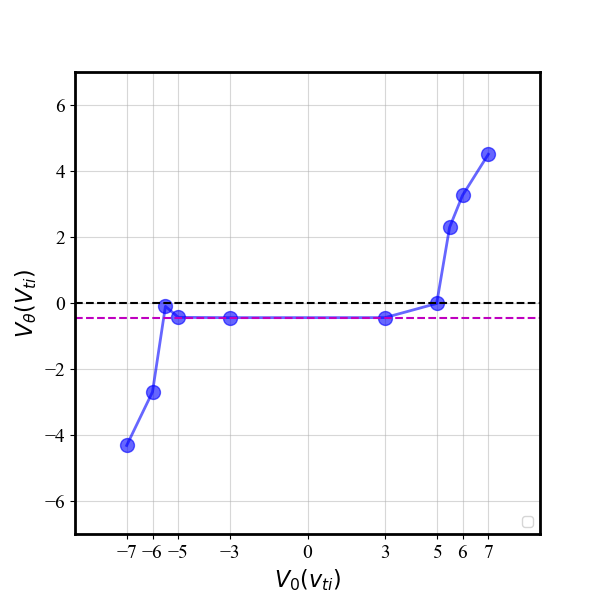
\includegraphics[width=0.35\textwidth]{../error_field/5f-1n0t/fix_n/sv_v.png}
		}
		\caption{}		
	\end{figure}
	1.紫线为抗磁性漂移速度的相反数
	2.由于密度剖面固定,抗磁性漂移速度不随时间演化,最后的电漂移和抗磁性大小相等,方向相反,加和为零。
	3.v=-5.5和5两个case应该时间没算够
	4.饱和状态不关于零点对称,但是由于抗磁性漂移较小,所以其实看起来影响不大

	\item 演化的密度剖面
	\begin{figure}[H]
		\centering
		\subfigure[磁岛宽度]{
			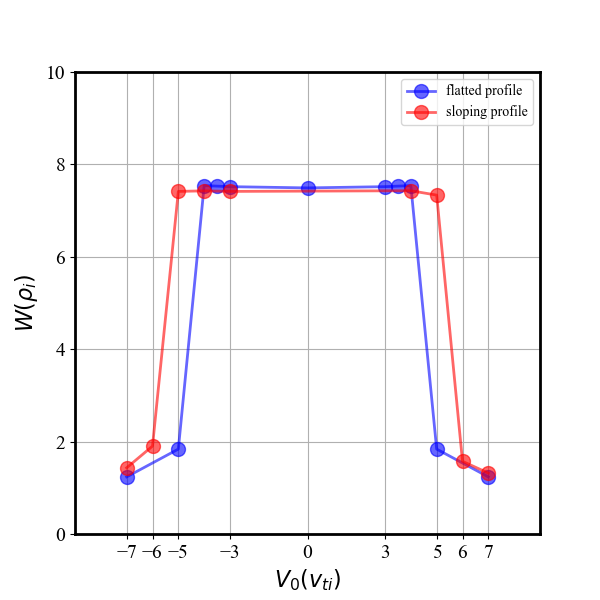
\includegraphics[width=0.35\textwidth]{../error_field/5f-1n0t/no_fix/sw_v.png} 
		}
		\subfigure[极向旋转]{
			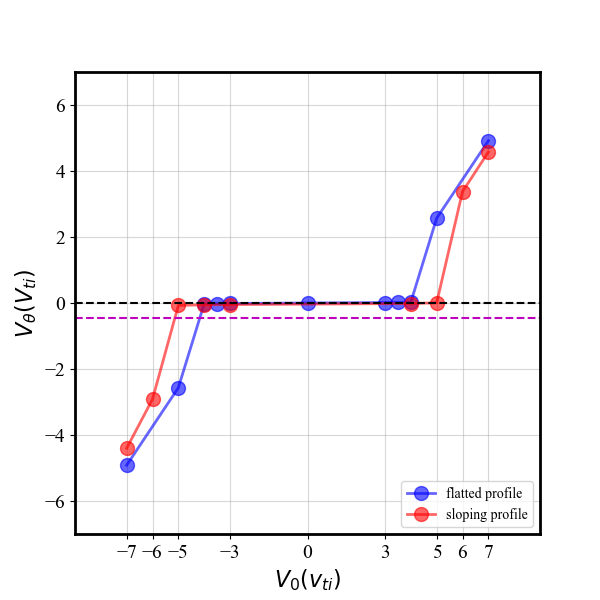
\includegraphics[width=0.35\textwidth]{../error_field/5f-1n0t/no_fix/sv_v.png}
		}
		\caption{}		
	\end{figure}
	1. 渗透的窗口扩大了(和一般的结论不太一样,一般的冷离子的模拟中窗口大小变化不大,主要是窗口的移动)
	2. 由于磁岛的形成导致密度剖面的展平,所以最后电漂移和抗磁性漂移都为零
\end{itemize}


\section{非平坦的温度剖面}
\subsection{不考虑湍流}
$$ n,T = 0.7 + 0.3(1-(r/a)^2)^2 $$
\begin{itemize}
	\item 固定的压强剖面
	\begin{figure}[H]
		\centering
		\subfigure[磁岛宽度]{
			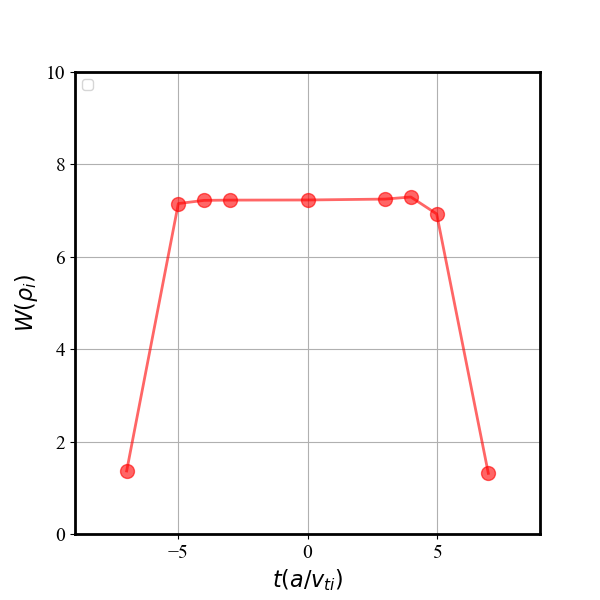
\includegraphics[width=0.35\textwidth]{../error_field/5f-1n1t/no_t/sw_v.png} 
		}
		\subfigure[极向旋转]{
			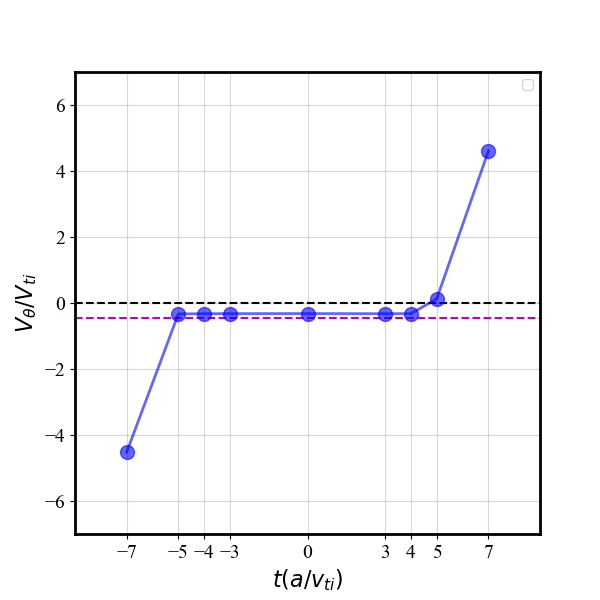
\includegraphics[width=0.35\textwidth]{../error_field/5f-1n1t/no_t/sv_v.png}
		}
		\caption{}		
	\end{figure}
	电漂移速度最终不等于电子密度梯度产生的抗磁性漂移速度,这个差值应该是电子朗道阻尼项起作用,和离子温度引起的抗磁性漂移有关,但是物理图像还不清楚
	
	\item 演化的压强剖面
	\begin{figure}[H]
		\centering
		\subfigure[磁岛宽度]{
			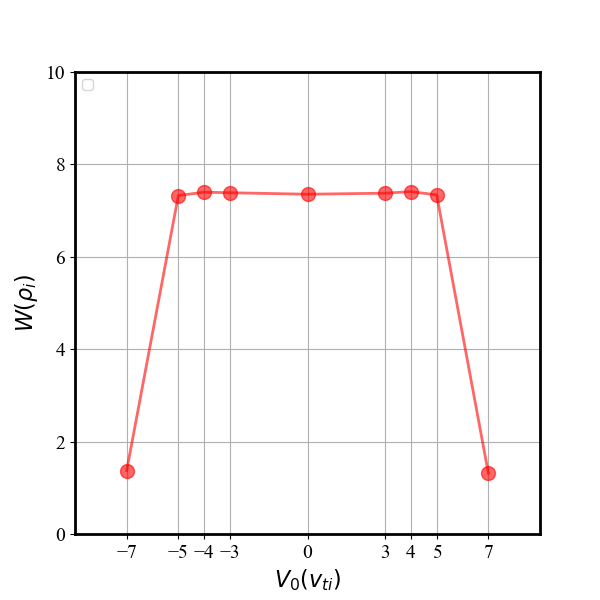
\includegraphics[width=0.35\textwidth]{../error_field/5f-1n1t/no_t/sw_v_1t.png} 
		}
		\subfigure[极向旋转]{
			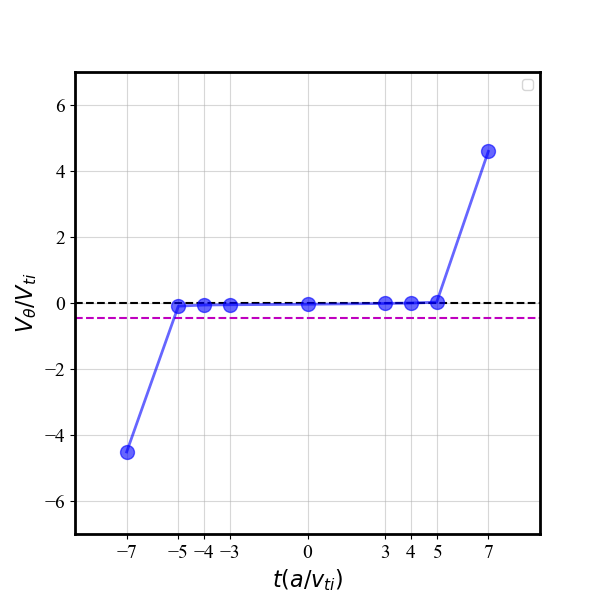
\includegraphics[width=0.35\textwidth]{../error_field/5f-1n1t/no_t/sv_v_1t.png}
		}
		\caption{}		
	\end{figure}
	电漂移速度最后等于零,固定剖面下稳态下电漂移对于密度梯度导致的抗磁性漂移的偏差可能是由于温度梯度导致的抗磁性漂移引起的,但是不太清楚怎么作用的。
\end{itemize}

\subsection{考虑湍流}

to be done...

\end{document}